\documentclass[10pt,a4paper]{article}
\usepackage[utf8]{inputenc}
\usepackage[spanish]{babel}
\usepackage[margin=1in]{geometry}
\usepackage{amsmath}
\usepackage{amsfonts}
\usepackage{amssymb}
\usepackage{enumitem}
\usepackage{hyperref} 
\usepackage{graphicx}
\usepackage{url}
\usepackage{breakurl}
\hypersetup{pdftex,colorlinks=true,allcolors=black}
\hypersetup{
    pdftitle={},
    pdfauthor={Pablo Riutort Grande},
    pdfsubject={},
    bookmarksnumbered=true,     
    bookmarksopen=true,         
    bookmarksopenlevel=1,       
    colorlinks=true,            
    pdfstartview=Fit,           
    pdfpagemode=UseOutlines,    % this is the option you were lookin for
    pdfpagelayout=TwoPageRight
}
\usepackage{listings}
\usepackage{xcolor}
\usepackage{hypcap}
\definecolor{codegreen}{rgb}{0,0.6,0}
\definecolor{codegray}{rgb}{0.5,0.5,0.5}
\definecolor{codepurple}{rgb}{0.58,0,0.82}
\definecolor{backcolour}{rgb}{0.95,0.95,0.92}
\lstdefinestyle{mystyle}{
    backgroundcolor=\color{backcolour},   
    commentstyle=\color{codegreen},
    keywordstyle=\color{magenta},
    numberstyle=\tiny\color{codegray},
    stringstyle=\color{codepurple},
    basicstyle=\ttfamily\footnotesize,
    breakatwhitespace=false,         
    breaklines=true,                 
    captionpos=b,                    
    keepspaces=true,                 
    numbers=left,                    
    numbersep=5pt,                  
    showspaces=false,                
    showstringspaces=false,
    showtabs=false,                  
    tabsize=2
}
\lstset{style=mystyle}
\usepackage{xparse}
\NewDocumentCommand{\codeword}{v}{%
\texttt{{#1}}
}
\author{Pablo Riutort Grande}
\title{PEC 4\\ \vspace{1cm}\textbf{Seguridad en los sistemas biométricos}}
\begin{document}
\maketitle
\pagebreak

\begin{enumerate}[label=\textbf{\alph*)}]
\item Después de mostrar el pasaporte, se registra la huella dactilar de uno de sus dedos y se toma una fotografía de la
cara. Esto correspondería al punto 1 de la figura del temario. De la misma forma, en las entradas de las salas de conferencias donde hay personal autorizado que realiza la identificación de los asistentes con ordenadores portátiles correpondería también al punto 1. En ambos se está haciendo uso de dispositivos lectores de datos biométricos.\\
Después de la toma de huellas en el primer punto de control, se envían las huellas y la fotografía a un ordenador que contiene el estractor de características (puntos 2 y 3), este esquema se corresponde al de la figura del temario.\\
Posteriormente, el extractor guarda en una base de datos remota los resultados. La base de datos remota se corresponde con el punto 6 del temario y la comunicación entre el estractor y la misma corresponden al punto 7.\\
Paralelamente, tenemos otro punto de acceso, las entradas de las salas de conferencia, que hacen tanto de punto 1 como de punto 9. La correspondencia con el punto 1 es debido a que en las entradas hay personal con ordenadores portátiles con dispositivos de medida biométrica y respecto al punto 9 es porque la sala es el recurso que se desea adquirir.\\
Los dispositivos biométricos de la entrada a la sala mandan las características al ordenador central de la universidad, que contiene el comparador (puntos 4 y 5). El ordenador central busca entonces en la base de datos (puntos 7 y 6) y devuelve al dispositivo la información de usuario (punto 8) encontrado: Si se ha encontrado o no y la fotografía del usuario en caso de que se haya encontrado.

\begin{figure}[h!]
  \centering
  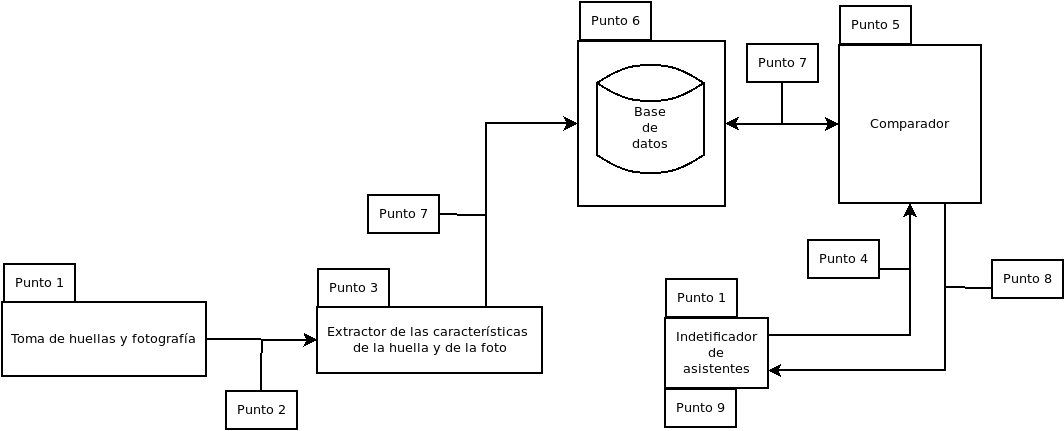
\includegraphics[scale=0.4]{diagram.png}\\
  \caption{Correspondencias con la Figura 1 del temario}
  \label{fig:puntos}
\end{figure}

\item
\begin{enumerate}[label=\textbf{\arabic*.}]
\item Los ataques de biometría falsa se basan en introducir datos falsos en el sensor, por tanto, se podrían producir únicamente en los puntos que corresponden al punto 1 porque es el único punto que contiene sensores biométricos.\\
Sería posible realizar un ataque de biometría falsa en estos desde el enfoque de la huella dactilar, puesto que ambos puntos de control están controlados por personal que podrían detectar fácilmente una técnica de ofuscación para el reconocimiento de cara. Para realizar un ataque directo de biometría falsa, en ese escenario, se podría crear una huella dactilar sintética que introduzca datos falsos en el sistema.
\item La inyección de paquetes falsos y los ataques de reenvío consisten en la captura de paquetes de datos procedentes de varios módulos del sistema y que viajan por algún canal de comunicación. Por tanto, este ataque únicamente podría realizarse a través de los puntos que interconectan otros puntos en el sistema: puntos 2, 4, 7 y 8.\\
Concretamente, en nuestro caso, atacar el punto 2 en ese esquema es extremadamente difícil puesto que en la primera toma de huellas los puntos 1 y 3 están separados por un punto 2 pero en la segunda toma este punto no existe porque el extractor de características está acoplado al mismo sistema que el sensor.\\
Los principales puntos de ataque en este esquema sean los puntos 7, introduciendo información falsa en la base de datos modificando las plantillas creadas de los usuarios. De manera similar, atacar al punto 4 alterando los datos provenientes del extractor de características con destino al módulo de comparación o se substituyéndolos por un conjunto nuevo de características podría ser factible, sin embargo, en este último proceso tendremos que estar seguros de los datos introducidos van a ser encontrados en la base de datos, de manera legítima o acompañado de un ataque al punto 7.\\
Finalmente, otra solución podría ser atacar el punto 8, donde nos centramos en atacar a cambiar el resultado final del proceso con el resultado deseado, independientemente de lo que haya en la base de datos o el veredicto del comparador.

\end{enumerate}

\item
Para prevenir un ataque de biometría falsa utilizando, por ejemplo, una huella dactilar sintética se pueden utilizar técnicas de detección de vida de la muestra. Estas técnicas consisten en medir la temperatura, el oxígeno, la conductividad de la piel y la detección de capilares bajo la epidermis o el pulso cardíaco.\\
Para prevenir ataques en los puntos relativos a la comunicación de componentes (puntos 2, 7, 4 y 8) se puede utilizar el cifrado cifrado de datos para prevenir el análisis de datos que circulan por el canal o la firma digital para evitar ataques del tipo \textit{man-in-the-middle}.\\
Adicionalmente, para proteger el punto 7 que contecta al comprador con la base de datos aumentaría el personal de seguridad para controlar el acceso físico a las instalaciones de la universidad.
\item 
Si el umbral de aceptación (A) es muy bajo entonces aumentaría la tasa de falsos aceptados y, por otra parte, si este umbral es muy alto entonces aumentaría la tasa de falsos rechazos.\\
En este caso, debido a la circunstancia de la comprobación de la fotografía del usuario aceptado por el sistema por parte de un humano, es preferible que el umbral A sea bajo para que haya más falsos aceptados. Aunque el sistema tenga más falsos aceptados, son los guardias los que verán en la foto si se trata de la persona o no en última instancia.\\
En caso contrario, si el umbral es alto, es decir, la tasa de falsos rechazos aumenta, el sistema solo dice que el usuario no tiene acceso y se podría vetar el acceso a personas que tienen legitimidad sobre el recurso.

\end{enumerate}

\end{document}